\documentclass{article}

\usepackage{neurips_2026}
% For anonymous submission use no options; for camera-ready use [main,final].

\usepackage[utf8]{inputenc}
\usepackage[T1]{fontenc}
\usepackage{hyperref}
\usepackage{url}
\usepackage{booktabs}
\usepackage{amsfonts}
\usepackage{amsmath}
\usepackage{nicefrac}
\usepackage{microtype}
\usepackage{xcolor}
\usepackage{graphicx}
\usepackage{multirow}
\usepackage{enumitem}
\usepackage{float}

\newcommand{\tbd}[1][]{{\color{red}\textbf{[TBD\if\relax#1\relax\else: #1\fi]}}}
\newcommand{\bodhi}{BODHI}
\newcommand{\hbhard}{HealthBench-Hard}
\newcommand{\affilsize}{\normalfont\fontsize{9}{11}\selectfont}

\title{Ask Before You Answer: Distilling Clinical Epistemic Calibration into Model Weights}

\author{Anonymous Author(s)}

\begin{document}
\raggedbottom

\maketitle

\begin{abstract}
How should we evaluate and instill the behaviors that distinguish calibrated expert reasoning from confident answer generation? Clarifying inquiry, scope bounding, principled abstention, and recognition of clinical warning signs are central to safe deployment in high-stakes domains, yet remain poorly measured and rarely targeted by current training pipelines. We contribute a framework for studying these epistemic behaviors as first-class objects of evaluation and design, and apply it to open-source clinical language models. The framework has three components. First, a seven-dimension behavioral decomposition (uncertainty acknowledgment, active inquiry, context-seeking, red-flag identification, scope bounding, hedging quality, specificity) that separates \emph{how} a model communicates from \emph{what} it knows, enabling claims about behavior that aggregate clinical scores obscure. Second, an asymmetric cross-family grading protocol (Qwen-14B as quality filter, Llama-8B as evaluator) that prevents filter-grader bias from inflating reported metrics, addressing a known failure mode in self-distillation pipelines. Third, a four-step pipeline for teaching epistemic behaviors to open-source models: a structured calibration reasoning protocol generates demonstrations, expert rubrics filter quality cases, and a LoRA adapter internalizes the behavior in the weights. Applied to MedGemma-27B on HealthBench with ${\sim}$3,100 filtered traces per seed, the resulting open-weight adapter raises active clinical inquiry from 17.5\% to 45.6\% ($d{=}0.63$, $n{\approx}1{,}000$), context-seeking from 1.40 to 1.75 on a 0--2 scale ($d{=}0.44$), red-flag identification from 1.52 to 1.67 ($d{=}0.20$), and scope bounding from 1.91 to 1.97 ($d{=}0.22$), with aggregate clinical quality preserved ($p{=}0.57$) and blanket disclaimers eliminated. We additionally surface a failure mode worth studying in its own right: combining the inference-time reasoning protocol with the adapted model degrades red-flag identification below the unadapted baseline, indicating that calibrated behavior interacts non-additively with inference-time scaffolding in ways current evaluation practices would miss. We release code, adapters, and the evaluation framework to support work on humble, uncertain, and inquiring open-source models.
\end{abstract}

%======================================================================
\section{Introduction}
\label{sec:intro}
%======================================================================

How should we build clinical language models that exhibit the behaviors of a careful expert? Not models that score well on multiple-choice benchmarks, but models that ask before answering, hedge when uncertain, name danger signs, and decline when they need more context. These behaviors---active inquiry, scope bounding, red-flag recognition, principled abstention---distinguish a calibrated expert from a confident guesser. They are also precisely what current training pipelines suppress, what current benchmarks fail to measure, and what we lack systematic methods to instill.

The problem has two parts: measurement and training. On measurement: aggregate clinical quality scores conflate \emph{what} a model knows with \emph{how} it communicates. A model can produce a clinically accurate response while omitting relevant uncertainty, failing to ask for missing context, or missing a warning sign that should trigger escalation; aggregate scores treat such a response as equivalent to a genuinely calibrated one. On training: language models trained with RLHF exhibit a systematic bias toward confident outputs \citep{kadavath2022language, lin2022teaching}. Human raters in preference labeling favor decisive responses over qualified ones \citep{xiong2024can}, and standard benchmarks reinforce this bias by scoring hedging and abstention as failures. The behaviors we want to encourage are penalized by the very objectives used to train and evaluate.

We use the term \emph{epistemic virtues} to refer to the behaviors that characterize calibrated expert reasoning: uncertainty acknowledgment, clarifying question-asking, scope bounding, evidence qualification, and principled abstention \citep{singhal2023medpalm, nori2023capabilities}. Building these behaviors into clinical models requires tools that can measure them precisely and training approaches that can target them directly.

Our starting point is the \bodhi{} protocol (\textbf{B}ridging, \textbf{O}pen, \textbf{D}iscerning, \textbf{H}umble, \textbf{I}nquiring) \citep{bodhi2026}, a structured chain-of-thought (CoT) protocol that forces a model through multi-step uncertainty analysis before generating a response. Pass~1 generates an internal analysis (clinical assessment, differentials, evidence quality, key uncertainties, questions to ask, scope boundaries, safe recommendations); Pass~2 generates a patient-facing response conditioned on that analysis. The CoT protocol reliably elicits the target epistemic behaviors at inference time, at $\sim$2$\times$ inference cost and with a $\sim$5\% response drop rate (context window exceeded). This makes it a useful demonstration source: run it on a large prompt set and you have a corpus of calibrated behavior at scale. It also makes it a poor deployment solution on its own---remove the CoT protocol and the model reverts.

This paper contributes a framework for studying epistemic behaviors as first-class objects of evaluation and design, and uses LoRA fine-tuning on CoT-generated demonstrations as evidence that the framework's behavioral dimensions are real, measurable, and respond to design interventions. The framework has three components: (1) a seven-dimension behavioral decomposition that separates \emph{how} a model communicates from \emph{what} it knows; (2) an asymmetric cross-family grading protocol that prevents filter-grader bias from inflating reported metrics; and (3) a recipe for teaching epistemic behaviors via CoT-conditioned demonstrations. Applied to MedGemma-27B \citep{medgemma2025} on 4,000 HealthBench \citep{healthbench2025} prompts with 5 independent seeds, the recipe produces LoRA adapters that shift multiple behavioral dimensions significantly without degrading clinical quality---demonstrating that the behavioral handles identified by the framework are actionable.

Our contributions:
\begin{enumerate}[leftmargin=*]
    \item An \textbf{epistemic virtue evaluation framework}: a seven-dimension behavioral decomposition (uncertainty acknowledgment, active inquiry, context-seeking, red-flag identification, scope bounding, hedging quality, specificity) that separates \emph{how} a model communicates from \emph{what} it knows, enabling claims about behavior that aggregate clinical scores obscure.
    \item An \textbf{asymmetric cross-family grading protocol}: Qwen-14B as quality filter, Llama-8B as evaluator, preventing filter-grader bias from inflating reported metrics---a known failure mode in self-distillation pipelines.
    \item \textbf{Evidence that the framework's behavioral dimensions respond to design}: quality-filtered SFT on \bodhi{} CoT demonstrations achieves active inquiry $d=0.63$, context-seeking $d=0.44$, scope bounding $d=0.22$, red-flag identification $d=0.20$, all $p < 10^{-5}$, $n\approx1{,}000$ per condition, with no degradation in aggregate clinical quality ($d=0.03$, $p=0.57$). The LoRA recipe is one concrete instantiation; the evaluation framework is what generalizes.
    \item \textbf{A design constraint revealed by the framework}: stacking the CoT protocol on the adapted model degrades red-flag identification below the unadapted baseline ($d=-0.25$, $p<10^{-7}$), indicating that CoT-induced and weight-based epistemic behaviors compete rather than compose---a finding invisible to aggregate evaluation.
\end{enumerate}

%======================================================================
\section{Related Work}
\label{sec:related}
%======================================================================

\paragraph{Calibration in language models.} \citet{kadavath2022language} demonstrated that LLMs possess internal uncertainty representations accessible via probing, but that RLHF-tuned outputs suppress this uncertainty. \citet{lin2022teaching} fine-tuned models on demonstrations with verbalized confidence (``I'm about 70\% sure...''), improving calibration on factual questions. \citet{tian2023just} showed similar effects from prompting alone. These works target \emph{numerical} confidence calibration. Our work targets \emph{behavioral} calibration: we do not ask the model to estimate its confidence as a number, but to modify its response behavior---hedging, questioning, abstaining---in ways appropriate to its uncertainty.

\paragraph{Medical LLM evaluation.} Standard medical benchmarks (MedQA, MMLU-Medical) evaluate factual accuracy via multiple-choice questions. HealthBench \citep{healthbench2025} differs by evaluating open-ended clinical responses against expert rubrics with both positive criteria (correct content, appropriate referrals) and negative criteria (dangerous advice, false reassurance, failure to escalate). This structure penalizes both overconfidence (meeting negative criteria) and excessive hedging (failing positive criteria for actionable guidance), making it suitable for evaluating calibrated behavior. We adopt the HealthBench grading protocol and extend it with prompt-injection hardening and cross-family grading.

\paragraph{Inference-time behavioral interventions.} Chain-of-thought prompting \citep{wei2022chain} improves reasoning by forcing intermediate steps. Constitutional AI \citep{bai2022constitutional} uses self-critique prompts to improve safety. \bodhi{} \citep{bodhi2026} uses a two-pass protocol: Pass~1 forces structured uncertainty analysis (clinical assessment, differentials, evidence quality, key uncertainties, questions to ask, scope boundaries, safe recommendations); Pass~2 generates a response conditioned on this analysis. The common limitation is deployment cost: the intervention must be applied at every inference call, consuming additional tokens and latency, with no guarantee that the underlying model has changed. We use the \bodhi{} CoT protocol not as the deployed intervention but as a demonstration source: the behavioral effect is distilled into model weights via fine-tuning, making the CoT protocol unnecessary at deployment.

\paragraph{LoRA and parameter-efficient fine-tuning.} LoRA \citep{hu2022lora} learns additive low-rank updates $\Delta W = BA$ with rank $r \ll \min(d,k)$. Variants include QLoRA \citep{dettmers2023qlora}, DoRA \citep{liu2024dora}, and rsLoRA \citep{kalajdzievski2023scaling}. LoRA is typically used for knowledge injection or task adaptation. We use it for \emph{behavioral modification}: the base model's knowledge is unchanged, but its manner of expressing that knowledge shifts toward calibrated uncertainty.

\paragraph{Self-improvement and behavioral distillation.} STaR \citep{zelikman2022star} bootstraps reasoning by filtering model-generated rationales on correctness; we apply the same filter-then-finetune logic to behavioral demonstrations rather than factual reasoning. Self-play fine-tuning \citep{chen2024selfplay} and iterative DPO \citep{yuan2024selfrewarding} improve capabilities through repeated self-sampling; we differ in using a \emph{structured CoT protocol} to shift the generation distribution rather than self-sampling from the base policy. Standard distillation \citep{hinton2015distilling} and chain-of-thought distillation \citep{ho2023large, magister2023teaching} transfer from a larger teacher model to a smaller student; here teacher and student are the \emph{same} model under different inference conditions. The key design insight is using the CoT protocol as a behavioral teacher: it imposes a structured output distribution at inference time, and the adapter internalizes that distribution, making the CoT protocol unnecessary at deployment.

%======================================================================
\section{Method}
\label{sec:method}
%======================================================================

\subsection{Overview}

Given a base model $M$, a structured CoT protocol $C$ that elicits target behaviors from $M$, and an evaluation rubric $R$ that can score the quality of $C(M)$'s outputs, the recipe proceeds in four steps:

\begin{enumerate}[leftmargin=*]
    \item \textbf{Generate}: Run $C(M)$ on a set of prompts $\mathcal{P}$ to produce demonstrations $\{(x_i, y_i)\}$.
    \item \textbf{Grade}: Score each demonstration $y_i$ against $R$, obtaining quality scores $\{s_i\}$.
    \item \textbf{Filter}: Retain demonstrations where $s_i \geq \tau$, yielding training set $\mathcal{D} = \{(x_i, y_i) : s_i \geq \tau\}$.
    \item \textbf{Distill}: Fine-tune $M$ on $\mathcal{D}$ with LoRA, producing $M + \Delta C$ that approximates $C(M)$'s behavior without $C$ at inference.
\end{enumerate}

The key assumption is that $C(M)$ produces outputs of varying quality, and that $R$ can distinguish successful demonstrations from failures. The filter step ensures the adapter trains only on demonstrations where the CoT protocol elicited the target behavior. We instantiate this with $M$ = MedGemma-27B-text-it, $C$ = \bodhi{} CoT protocol, $R$ = HealthBench expert rubrics, $\tau = 0.4$, and $\Delta C$ = LoRA ($r{=}16$). Figure~\ref{fig:pipeline} shows the full pipeline and the $2{\times}2$ evaluation design.

\begin{figure}[t]
\centering
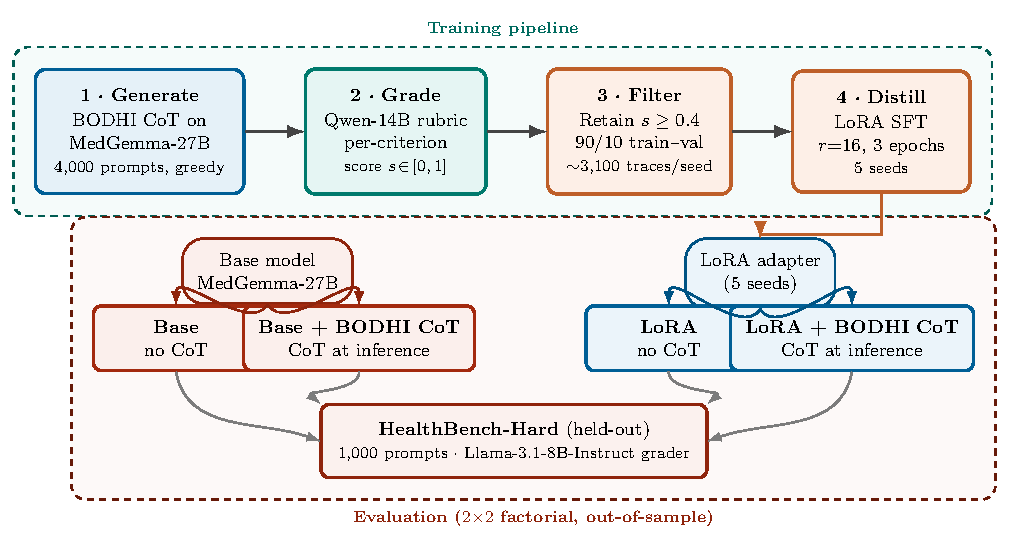
\includegraphics[width=\linewidth]{figures/pipeline.pdf}
\caption{Overview of the training pipeline (top) and evaluation design (bottom). The training pipeline follows four steps: generate demonstrations via the \bodhi{} CoT protocol, grade against HealthBench rubrics using Qwen-14B, filter to quality traces ($s\geq0.4$), and distill into a LoRA adapter. The evaluation uses a $2{\times}2$ factorial design: base model with and without the CoT protocol, and LoRA adapter with and without the CoT protocol, all evaluated on the held-out HealthBench-Hard set (1,000 prompts). The CoT protocol is \emph{not required} at deployment for the LoRA condition.}
\label{fig:pipeline}
\end{figure}

\subsection{Trace Generation}

We apply \bodhi{}'s two-pass CoT protocol to MedGemma-27B-text-it on prompts from HealthBench Full (${\sim}$5,000 prompts). HealthBench Hard is a strict subset of HealthBench Full; we exclude all 1,000 Hard prompts by \texttt{prompt\_id} matching, yielding 4,000 generation prompts. This exclusion is enforced at generation time and independently re-verified by an automated preflight gate before every training job.

Inference uses vLLM \citep{kwon2023efficient} with tensor parallelism across $8\times$ TPU v6e chips (256\,GB HBM), greedy decoding (temperature 0) for determinism, and 32 concurrent requests via continuous batching. Each trace records the input messages, the \bodhi{} Pass~1 analysis (the model's internal uncertainty reasoning), and the Pass~2 response (the patient-facing text). The analysis field is not used during training---only the response is---but is retained for post-hoc inspection of where the CoT protocol's reasoning succeeded or failed.

\subsection{Rubric Grading and Filtering}

Not all CoT-generated outputs are high-quality. The CoT protocol occasionally produces over-hedged responses, incoherent analyses, or responses that fail rubric criteria despite the structured analysis. We grade each trace against HealthBench's expert-authored rubrics and retain only strong demonstrations.

A grader LLM (Qwen/Qwen2.5-14B-Instruct) evaluates each rubric criterion independently, producing a boolean \texttt{criteria\_met} judgment per criterion. We compute a normalized score:
\begin{equation}
    s = \frac{p_{\text{earned}} - p_{\text{neg}}}{p_{\text{pos}} - p_{\text{neg}}}
    \label{eq:score}
\end{equation}
where $p_{\text{pos}}$ and $p_{\text{neg}}$ are the sums of positive and negative rubric points and $p_{\text{earned}}$ is the sum of points for criteria met. This bounds $s \in [0,1]$ and normalizes across prompts with different numbers of criteria. Traces with $s \geq 0.4$ are retained, yielding ${\sim}$3,100 traces per seed (${\sim}$2,800 train / ${\sim}$310 validation after a seeded 90/10 split). The threshold $\tau=0.4$ was chosen at the 25th percentile of pilot scores on 500 traces, excluding the lowest-quality quarter of CoT-generated outputs. The ${\sim}$78\% retention rate (3,129 of 4,000 prompts) confirms the filter removes a meaningful tail of failures rather than discarding rare successes.

\paragraph{Asymmetric grader design.} The choice of Qwen-14B as filter grader is deliberate: the evaluation grader (\S\ref{sec:eval}) is Llama-3.1-8B-Instruct, a different model family. This asymmetry ensures that any Qwen-specific grading bias affects only which traces enter training, not the reported evaluation scores. The evaluator that determines the reported numbers never participated in training data selection.

\paragraph{Prompt-injection hardening.} The HealthBench grading template interpolates untrusted trace content between delimiter markers (\texttt{<<conversation>>}) and uses section headers (\texttt{\# Final instruction}). An adversarial response containing these literal strings could manipulate grading decisions. We escape all template delimiters in interpolated content before grading. This is mitigation rather than full prevention, but raises the bar for adversarial manipulation without changing the semantics of legitimate clinical text.

\subsection{LoRA Fine-Tuning}

We fine-tune MedGemma-27B with LoRA ($r{=}16$, $\alpha{=}32$, dropout 0.05) targeting all linear projections in attention and MLP layers (q, k, v, o, gate, up, down---7 module types per layer). Training uses \textbf{completion-only loss masking}: the cross-entropy loss is computed only on assistant response tokens, with all prompt and user tokens masked. This focuses the gradient on generating calibrated responses rather than memorizing prompt structure or user messages.

Hyperparameters: 3 epochs, effective batch size 16 (2 per device $\times$ 8 gradient accumulation steps), learning rate $10^{-4}$ with cosine schedule and 5\% warmup, bfloat16 precision. On TPU, the 27B base model (54\,GB in bf16) is sharded across 8 chips via FSDPv2, wrapping each \texttt{Gemma3DecoderLayer} in an FSDP unit under a single-process SPMD configuration.

We train 5 independent adapters with seeds 42, 7, 13, 99, and 101, varying LoRA weight initialization, data shuffling order, and dropout masks. All results are reported as mean $\pm$ std across these 5 seeds. Full hyperparameter configuration is in Appendix~\ref{app:hparams}.

\subsection{Evaluation}
\label{sec:eval}

\paragraph{Test set.} For each seed $k$, we draw 200 prompts without replacement from the 1,000 \hbhard{} examples. All 1,000 Hard prompts are excluded from training, so every possible 200-prompt draw is out-of-sample. The per-seed repeated subsampling captures both training noise (different LoRA init and data order) and eval-set-choice noise (different 200 prompts) in the reported variance.

\paragraph{Configurations.} We evaluate four conditions per seed in a $2 \times 2$ factorial design: Base, Base+\bodhi{} CoT, LoRA (no CoT), and LoRA+\bodhi{} CoT. This isolates the CoT effect on the base model (Base $\to$ Base+\bodhi{}), the weight-based effect of fine-tuning (Base $\to$ LoRA), the residual CoT value after fine-tuning (LoRA $\to$ LoRA+\bodhi{}), and potential interference between the two mechanisms.

\paragraph{Grading.} The evaluation grader is Llama-3.1-8B-Instruct. Evaluation was conducted on A100-80GB GPUs via Modal, with MedGemma-27B and the LoRA adapter merged on CPU before serving.

\paragraph{Epistemic virtue decomposition.} A separate evaluation pass grades each response on seven behavioral dimensions: (1) uncertainty acknowledgment (0--2), (2) active inquiry (binary question-asking rate), (3) context-seeking (0--2, substantiveness of questions), (4) red-flag identification (0--2), (5) scope bounding (0--2), (6) specificity (0--2), and (7) hedging quality (appropriate vs.\ blanket disclaimer). This decomposition distinguishes \emph{which} specific behaviors the adapter induces, beyond aggregate score changes.

The blanket-disclaimer rate is the key diagnostic for the ``hedging trap'': a model that has learned genuine calibration will have high appropriate-hedging rate and low blanket-disclaimer rate, while a model that has learned indiscriminate caution will have both rates high.

\paragraph{Integrity controls.} (1)~A contamination probe (Appendix~\ref{app:contamination}) on 105 \hbhard{} prompts found zero verbatim memorization (0/105 exact-match completions, mean prefix-overlap $=0$ tokens), consistent with no pretraining contamination. (2)~An automated leakage gate verifies that no evaluation prompt IDs appear in training data. (3)~Grader parse-failure rate is monitored ($<0.1\%$ across all reported runs); on parse failure the criterion is marked as not-met (conservative), and the retry loop operates under the same token budget as the original call, so retry success is not expected and failures do not silently inflate scores. (4)~Physician validation of the LLM grader is pre-registered and in progress (Appendix~\ref{app:human}); aggregate-quality claims should be read as rubric-based proxy quality until those grades return.

%======================================================================
\section{Results}
\label{sec:results}
%======================================================================

\subsection{Main Results}

\begin{table}[t]
\centering
\caption{\hbhard{} normalized rubric scores (Eq.~\ref{eq:score}). 5-seed repeated subsampling, 200 prompts per seed. Grader: Llama-3.1-8B-Instruct. Mean and 95\% CI across seeds. $n$: mean responses graded per seed (out of 200). No pairwise comparison reaches significance ($\alpha=0.05$).}
\label{tab:main}
\begin{tabular}{lccc}
\toprule
Config & Score (mean) & 95\% CI & $n$/seed \\
\midrule
Base & 0.459 & [0.445,\;0.473] & 200 \\
Base + \bodhi{} & 0.463 & [0.450,\;0.476] & 191 \\
LoRA (no CoT) & 0.463 & [0.451,\;0.475] & 200 \\
LoRA + \bodhi{} & 0.455 & [0.453,\;0.457] & 192 \\
\bottomrule
\end{tabular}
\end{table}

Table~\ref{tab:main} presents aggregate scores. The aggregate score is \emph{not} the primary claim---it establishes a non-inferiority constraint: the adapter does not degrade clinical quality ($d=0.03$, $p=0.57$, $n\approx1{,}000$ prompts per condition). Three features of the aggregate results warrant attention.

\textbf{Clinical quality is preserved.} No pairwise comparison reaches significance at $\alpha=0.05$. The adapter modifies \emph{how} the model communicates, not \emph{what} it knows.

\textbf{The CoT protocol drops 5\% of responses.} Both CoT conditions (Base+\bodhi{}, LoRA+\bodhi{}) fail to produce a response for $\sim$5\% of prompts because the two-pass analysis exceeds the 4,096-token context window. The LoRA adapter has a 100\% response rate.

\textbf{LoRA+\bodhi{} scores lowest.} At $0.455$ it is below both LoRA ($0.463$) and Base+\bodhi{} ($0.463$). The effect is not significant ($p=0.15$) but the cross-seed variance is strikingly low ($\sigma=0.002$), suggesting the interference is systematic.

\subsection{Epistemic Virtue Decomposition}

\begin{table}[t]
\centering
\caption{Epistemic virtue scores (5-seed mean $\pm$ std). Top: graded on 0--2 scale (cross-seed std omitted; all ${\leq}0.03$). Bottom: rates with cross-seed std as subscript. $\downarrow$ indicates lower is better.}
\label{tab:epistemic}
\begin{tabular}{lcccc}
\toprule
Dimension & Base & +\bodhi{} & LoRA & LoRA+\bodhi{} \\
\midrule
Uncertainty ack.\ (0--2) & 1.94 & 1.90 & 1.94 & 1.95 \\
Context-seeking (0--2) & 1.40 & 1.77 & 1.75 & 1.90 \\
Red-flag identification (0--2) & 1.52 & 1.66 & 1.67 & 1.51 \\
Scope bounding (0--2) & 1.91 & 1.94 & 1.97 & 1.98 \\
Hedging quality (0--2) & 1.86 & 1.85 & 1.91 & 1.91 \\
Specificity (0--2) & 1.88 & 1.88 & 1.92 & 1.92 \\
\midrule
Questions / response & $0.45_{\pm.11}$ & $1.25_{\pm.08}$ & $1.16_{\pm.14}$ & $1.71_{\pm.12}$ \\
Active inquiry rate & $17.5_{\pm3.3}$\% & $47.9_{\pm2.9}$\% & $45.6_{\pm3.9}$\% & $80.0_{\pm6.7}$\% \\
Red-flag rate & $72.4_{\pm0.8}$\% & $78.8_{\pm2.1}$\% & $78.3_{\pm2.0}$\% & $57.7_{\pm8.0}$\% \\
Scope bounded rate & $92.7_{\pm1.1}$\% & $95.4_{\pm1.5}$\% & $97.6_{\pm0.7}$\% & $98.1_{\pm1.5}$\% \\
Specificity rate & $61.2_{\pm3.9}$\% & $61.4_{\pm4.0}$\% & $61.2_{\pm4.3}$\% & $65.0_{\pm2.3}$\% \\
Blanket disclaimer $\downarrow$ & $0.5_{\pm0.4}$\% & 0.0\% & 0.0\% & 0.0\% \\
Appropriate hedging & $90.6_{\pm1.7}$\% & $91.7_{\pm1.7}$\% & $94.2_{\pm1.6}$\% & $94.9_{\pm1.5}$\% \\
\bottomrule
\end{tabular}
\end{table}

\begin{figure}[t]
\centering
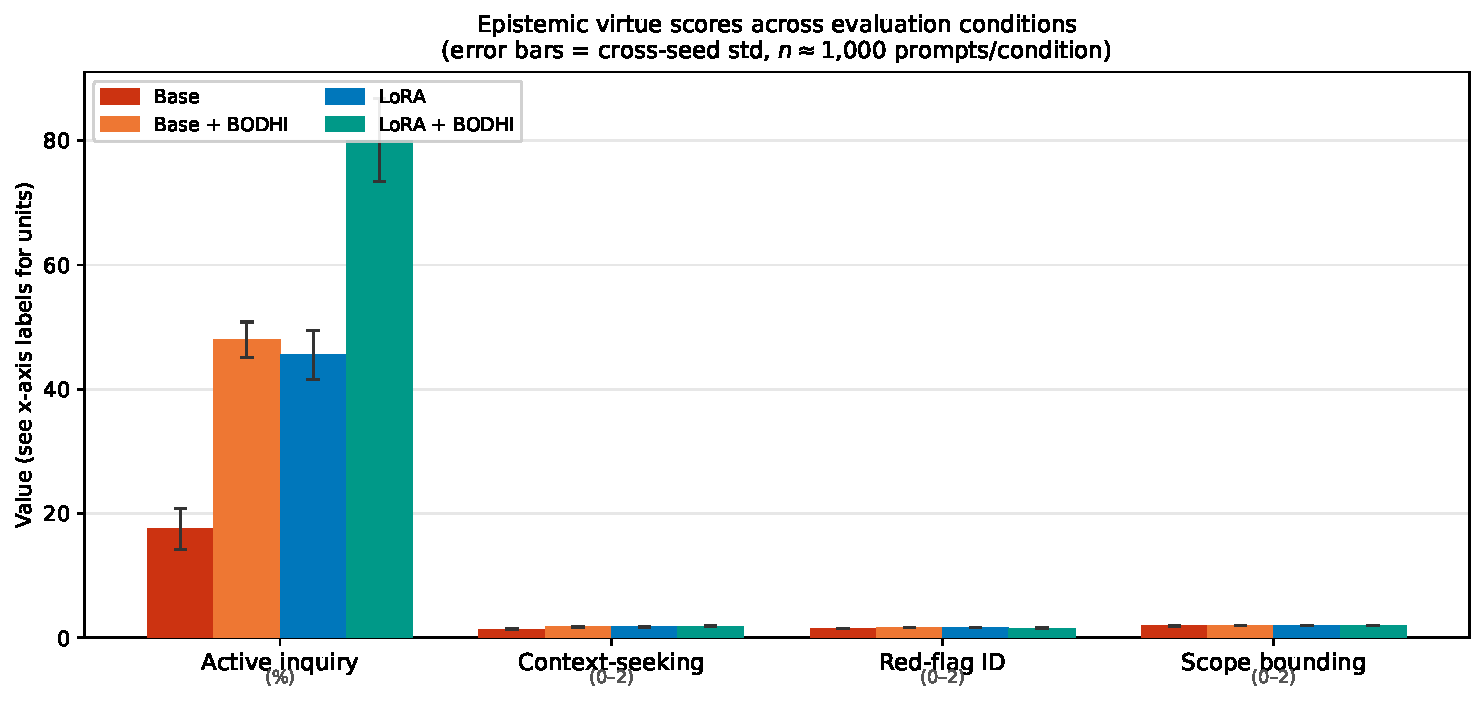
\includegraphics[width=\linewidth]{figures/epistemic_bar.pdf}
\caption{Epistemic virtue scores across the four evaluation conditions. Error bars show cross-seed standard deviation ($n{=}5$ seeds, ${\approx}200$ prompts per seed per condition). Active inquiry and context-seeking increase substantially with the LoRA adapter; red-flag identification regresses when the CoT protocol is stacked on the adapter (LoRA+BODHI CoT), dropping below the unadapted base. Per-seed consistency is shown in Appendix~\ref{app:perseed}.}
\label{fig:epistemic_bar}
\end{figure}

Table~\ref{tab:epistemic} and Figure~\ref{fig:epistemic_bar} show where the behavioral change occurs. Effect sizes for all seven dimensions are summarized in Appendix~\ref{app:forest}. All statistics below use prompt-level two-sample $t$-tests ($n\approx985$--$998$ per condition, pooled across 5 seeds; seeds draw without replacement within-seed but independently across seeds, introducing some prompt overlap, though p-values are far below any threshold where this matters). All p-values are uncorrected for multiple comparisons; Bonferroni correction over the reported comparisons does not change any binary significance conclusion given effect sizes $d \geq 0.20$ throughout.

\textbf{Active inquiry.} The largest effect. Base asks clarifying questions in 17.5\% of responses (0.45 questions per response). The LoRA adapter raises this to 45.6\% (1.16 questions/response), closely matching the CoT protocol's 47.9\% ($d = 0.63$, $p < 10^{-40}$). By Cohen's conventions this is a medium-to-large effect ($d=0.63$ exceeds the medium threshold of 0.5)---meaningful given that prompts within a condition vary substantially in difficulty and topic.

\textbf{Context-seeking.} The context-seeking score rises from 1.40 to 1.75 on the 0--2 scale ($d = 0.44$, $p < 10^{-20}$), capturing not just whether the model asks questions but how substantive they are.

\textbf{Scope bounding.} The adapter exceeds the CoT protocol: 97.6\% vs.\ 95.4\% (base: 92.7\%, $d = 0.22$, $p < 10^{-5}$).

\textbf{Appropriate hedging.} The blanket-disclaimer rate drops to 0.0\% (base: 0.5\%) and hedging quality rises from 1.86 to 1.91. The adapter produces targeted, contextually appropriate hedging rather than generic boilerplate.

\textbf{Red-flag identification.} The adapter raises red-flag identification from 1.52 to 1.67 on the 0--2 scale ($d = 0.20$, $p < 10^{-5}$). This safety-critical behavior---recognizing clinical warning signs that require escalation---transfers reliably to the adapted weights.

\textbf{Specificity is preserved.} The specificity rate is unchanged at 61.2\%, indicating the adapter does not sacrifice concrete clinical content (dosages, timeframes, referral specifics) in exchange for increased hedging. The model has not learned to replace substance with qualifications.

\textbf{Uncertainty acknowledgment.} Unexpectedly, the \bodhi{} CoT protocol modestly reduces uncertainty acknowledgment (Base: 1.94 $\to$ Base+\bodhi{}: 1.90), while the LoRA adapter leaves it unchanged (1.94). One possible explanation is that the CoT protocol's analysis pass reformulates uncertainty within the internal reasoning rather than foregrounding it in the patient-facing response. We flag this as an unresolved finding that warrants analysis of the Pass~1 analysis-field content.

\textbf{CoT--adapter interference.} When the CoT protocol is applied on top of the adapted model, active inquiry rises further to 80.0\%---but red-flag identification drops from 1.67 to 1.51 ($d = -0.25$, $p < 10^{-7}$), \emph{below} the unadapted base (1.52). The CoT protocol's analysis pass consumes context that the adapter's learned patterns would otherwise use for red-flag recognition. This is the clearest evidence of internalization: the two mechanisms compete for the same behavioral capacity.

\subsection{Response Characteristics}

Base model responses average ${\sim}$3,220 characters. The LoRA adapter produces longer responses (${\sim}$3,410 characters, $+5.9$\%), accounted for by additional clarifying questions and scope-bounding language. A 190-character increase cannot account for a 28-percentage-point rise in active inquiry: the behavioral shift is qualitative, not a verbosity artifact.

By contrast, the \bodhi{} CoT protocol produces substantially longer responses: ${\sim}$4,080 characters for Base+\bodhi{} ($+27$\%) and ${\sim}$6,190 characters for LoRA+\bodhi{} ($+92$\%), because the two-pass analysis leaks into patient-facing text. The adapter achieves the CoT protocol's behavioral effect at less than a quarter of the length overhead.



%======================================================================
\section{Discussion}
\label{sec:discussion}
%======================================================================

\paragraph{What the framework makes visible.} The aggregate score is not what this paper is about---the adapter does not improve HealthBench-Hard scores ($d=0.03$, $p=0.57$). What the framework makes visible is that the adapter induces consistent, statistically significant shifts in \emph{specific epistemic behaviors} (Table~\ref{tab:epistemic}, Figure~\ref{fig:epistemic_bar}) at the prompt level: active inquiry ($d=0.63$), context-seeking ($d=0.44$), scope bounding ($d=0.22$), red-flag identification ($d=0.20$), all $p < 10^{-5}$, $n\approx1{,}000$ per condition---while leaving aggregate clinical quality unchanged. These are not the same claim. An aggregate score that is unchanged can mask large behavioral shifts in either direction; a framework that decomposes behavior dimension by dimension cannot. Stacking the CoT protocol on the adapter degrades red-flag identification below the unadapted baseline ($d=-0.25$, $p < 10^{-7}$): a finding that is invisible to aggregate evaluation and legible only through the behavioral decomposition.

\paragraph{Calibration, not hedging.} A key concern with any approach that increases uncertainty expression is whether the model has learned calibrated behavior or indiscriminate caution. Four observations argue for calibration. (1)~The blanket-disclaimer rate drops to 0.0\%---the adapter produces targeted hedging, not generic qualifications. (2)~Specificity is preserved at 61.2\%---the adapter does not sacrifice concrete clinical content for vagueness. (3)~The appropriate-hedging rate increases from 90.6\% to 94.2\%---more hedging occurs, but it is contextually appropriate. (4)~Response length increases by 5.7\% (+190 characters), which cannot account for a 28~pp shift in active inquiry rates. A difficulty stratification (Appendix~\ref{app:ushape}) shows that failure rates rise monotonically with prompt difficulty across all conditions, with no condition clearly dominating across the full difficulty range---consistent with the adapter modifying \emph{how} the model communicates rather than improving its underlying clinical knowledge.

\paragraph{CoT--adapter interference as a design constraint.} The LoRA+\bodhi{} result reveals a design constraint. Red-flag identification drops from 1.67 (LoRA alone) to 1.51 (LoRA+\bodhi{}, $d=-0.25$, $p<10^{-7}$)---\emph{below} the unadapted base model (1.52)---even as active inquiry rises to 80.0\%. The CoT protocol's analysis pass competes with the adapter's learned red-flag patterns for the model's attention budget. The framework makes this constraint legible: without the behavioral decomposition, the aggregate score would show a small non-significant drop and the interference would go undiagnosed. If an adapted model is deployed, the CoT protocol must be removed---stacking them is not a safety net, it is a regression. A pre-registered harm-potential analysis (Appendix~\ref{app:harm}) is in progress to quantify whether the regression manifests in clinically harmful responses.

\paragraph{Self-distillation and grader sensitivity.} A methodological concern is that the LoRA adapter is trained on MedGemma-27B's own outputs and evaluated on MedGemma-27B's outputs, graded by a third-party LLM. This creates a closed loop: the adapter may learn to produce outputs that the Llama-8B grader scores similarly, without genuinely improving clinical behavior. We note two mitigating factors: (1) the epistemic virtue decomposition measures behavioral properties (question-asking, scope bounding) that are less susceptible to grader-style artifacts than aggregate scores; (2) the active-inquiry shift ($d=0.63$, $p<10^{-40}$, $n\approx1{,}000$) involves a concrete observable behavior that is difficult to attribute to grader stylistic preference. We additionally note a grader-sensitivity signal: in an earlier result set graded by Qwen-14B as evaluator (rather than Llama-8B), the aggregate score pattern showed small sign changes ($|\Delta|<0.01$). This is consistent with the self-distillation concern and reinforces that the physician validation in progress (Appendix~\ref{app:human}) is the definitive assessment.

\paragraph{Scope and generality.} This paper validates one instantiation: \bodhi{} CoT protocol, LoRA fine-tuning, MedGemma-27B, medicine, HealthBench. The framework does not depend on any of these choices. Any structured CoT protocol that elicits scorable behavioral demonstrations can serve as the generation step. Any parameter-efficient fine-tuning method can serve as the distillation step. The seven-dimension behavioral decomposition can be adapted to any domain where calibrated expert behavior can be operationalized. The asymmetric grading protocol applies to any self-distillation pipeline. What this paper establishes is that the framework's behavioral dimensions are real, measurable, and respond to design---on one concrete instantiation, at scale. Whether the specific effect sizes generalize, whether other CoT protocols produce the same interference pattern, and whether the recipe transfers to other domains are the important next questions.

\paragraph{Limitations.} (1)~\textbf{Single-setting scope}: one model, one CoT protocol, one domain, one benchmark. Effect sizes and interference patterns may not generalize. (2)~\textbf{LLM-as-judge}: evaluation uses Llama-3.1-8B-Instruct; human expert validation (Appendix~\ref{app:human}) is in progress and will provide the definitive quality assessment. (3)~\textbf{Self-distillation}: the adapter is trained on the base model's own outputs; the adapter may have learned to satisfy the Llama grader's stylistic preferences rather than genuinely improving clinical behavior. The large active-inquiry shift ($d=0.63$, $p<10^{-40}$) is hard to explain as a grader artifact, but human evaluation is needed to confirm. (4)~\textbf{Greedy decoding only}: behavior under sampling is untested. (5)~\textbf{No ablations}: filter threshold $\tau$, LoRA rank, and training set size are untested open questions; component ablations require additional compute beyond the current budget. (6)~\textbf{Truncation normalizes traces}: the 4,096-token context window drops CoT-generated responses that exceed it ($\sim$5\%). Because long responses are more likely to fail the window check, the training set over-represents responses that fit within the limit. This forces similarity across training traces independent of behavioral quality, meaning that score improvements cannot be attributed solely to longer or richer responses---the truncation itself acts as a normalizing filter and prevents attribution of gains to verbosity alone.

%======================================================================
\section{Conclusion}
\label{sec:conclusion}
%======================================================================

We contribute a framework for evaluating epistemic behaviors as first-class design targets in clinical language models, and demonstrate via LoRA fine-tuning on \bodhi{} CoT-generated demonstrations that the framework's behavioral dimensions respond to design interventions. Applied to MedGemma-27B on HealthBench-Hard, the recipe produces open-weight adapters that shift active inquiry by $+28$~pp ($d=0.63$, $p<10^{-40}$), context-seeking by $+0.35$ on a 0--2 scale ($d=0.44$), red-flag identification by $+0.15$ ($d=0.20$), and scope bounding by $+0.06$ ($d=0.22$), while leaving aggregate clinical quality unchanged ($d=0.03$, $p=0.57$) and eliminating blanket disclaimers. The framework additionally surfaces a design constraint invisible to aggregate evaluation: stacking the CoT protocol on the adapted model degrades red-flag identification \emph{below} the unadapted baseline ($d=-0.25$, $p<10^{-7}$), indicating that CoT-induced and weight-based epistemic behaviors compete for the same behavioral capacity.

The practical upshot is a recipe: identify a CoT protocol that elicits the target epistemic behaviors, generate demonstrations at scale, grade and filter with an asymmetric cross-family grader, fine-tune with LoRA, and use the seven-dimension decomposition to verify that the right behaviors shifted. The recipe is not tied to \bodhi{}, MedGemma, or HealthBench. Code, adapters, and the evaluation framework are at \url{https://anonymous.4open.science/r/bodhi-lora-CEB5}.

\begin{ack}
Funding: None declared.
\end{ack}

\bibliographystyle{unsrtnat}
\bibliography{references}

\clearpage
\appendix
\raggedbottom

\section{Contamination Probe}
\label{app:contamination}

We test whether MedGemma-27B has memorized \hbhard{} prompts during pretraining. The protocol feeds the base model the first 15 tokens of each Hard prompt and asks for a 25-token continuation, then measures (a)~the exact-completion rate against the ground-truth continuation and (b)~the mean prefix-overlap in tokens. A second probe on PubMedQA questions provides a length-matched control distribution.

Of 200 Hard prompts sampled, 105 met the minimum-length requirement (prompt $\ge 40$ tokens). On those 105 prompts, the model produced \emph{zero} exact-match completions and a mean prefix-overlap of \emph{zero} tokens. The PubMedQA control probe produced no usable samples because PubMedQA questions are typically 10--20 tokens, below the 40-token threshold; we report the absolute zero on \hbhard{} alone and note the control baseline as a length-mismatch limitation. The headline finding---no detectable verbatim memorization on the prompts where the probe is well-defined---is consistent with no contamination. The probe data and per-prompt outputs are available with the rest of the artifacts.

\section{Human Expert Validation}
\label{app:human}

Physician validation of the LLM grader is in progress. The protocol pre-registered for this study: 50 responses per configuration (200 eval total) plus 100 Qwen-graded filter traces, expanded to per-criterion grading rows; 3 board-certified physicians score each criterion blind to the response source on a $\{$pass, fail, unsure$\}$ scale with three confidence levels; a fourth adjudicator resolves criteria where the three reviewers gave three different grades. We report quadratic-weighted Cohen's $\kappa$ between (i)~each pair of physicians and (ii)~physician consensus and the LLM grader, separately for the Llama-3.1-8B eval grader and the Qwen-14B filter grader, and broken out by the four Stage-4 conditions. Target: $\kappa \geq 0.6$ vs.\ physician consensus. The grading sheets are out at the time of submission and we will report results when the reviews return; until then, all aggregate-quality claims should be read as \emph{rubric-based proxy quality with LLM-as-judge}, not as settled clinical validation. We treat this as a known limitation and a pre-registered next step rather than a completed integrity control.

\section{Harm-Potential Analysis}
\label{app:harm}

Clinician review of high-stakes prompts is not yet completed and remains a pre-registered limitation. The intended protocol: identify HBHard prompts in four high-stakes categories (chest pain triage, anaphylaxis, suicide risk, drug-allergy contraindications), and have clinicians grade whether the response causes harmful delay-to-care relative to a base-model reference. Until those grades return, the central methodological risk---that the adapter trains the model to hedge in cases where confident, direct response would be clinically appropriate---cannot be ruled out. We flag the \emph{LoRA+\bodhi{}} red-flag-identification regression (57.7\% vs.\ 78.3\% for LoRA alone) as an early warning sign that motivates this analysis.

\section{Per-Seed Results}
\label{app:perseed}

\begin{table}[t]
\centering
\caption{Per-seed \hbhard{} scores (Eq.~\ref{eq:score}).}
\begin{tabular}{lccccc}
\toprule
Config & Seed 7 & Seed 13 & Seed 42 & Seed 99 & Seed 101 \\
\midrule
Base & 0.459 & 0.453 & 0.472 & 0.443 & 0.467 \\
Base + \bodhi{} & 0.479 & 0.457 & 0.460 & 0.467 & 0.452 \\
LoRA & 0.475 & 0.449 & 0.468 & 0.463 & 0.461 \\
LoRA + \bodhi{} & 0.456 & 0.457 & 0.457 & 0.456 & 0.452 \\
\bottomrule
\end{tabular}
\end{table}

\begin{figure}[H]
\centering
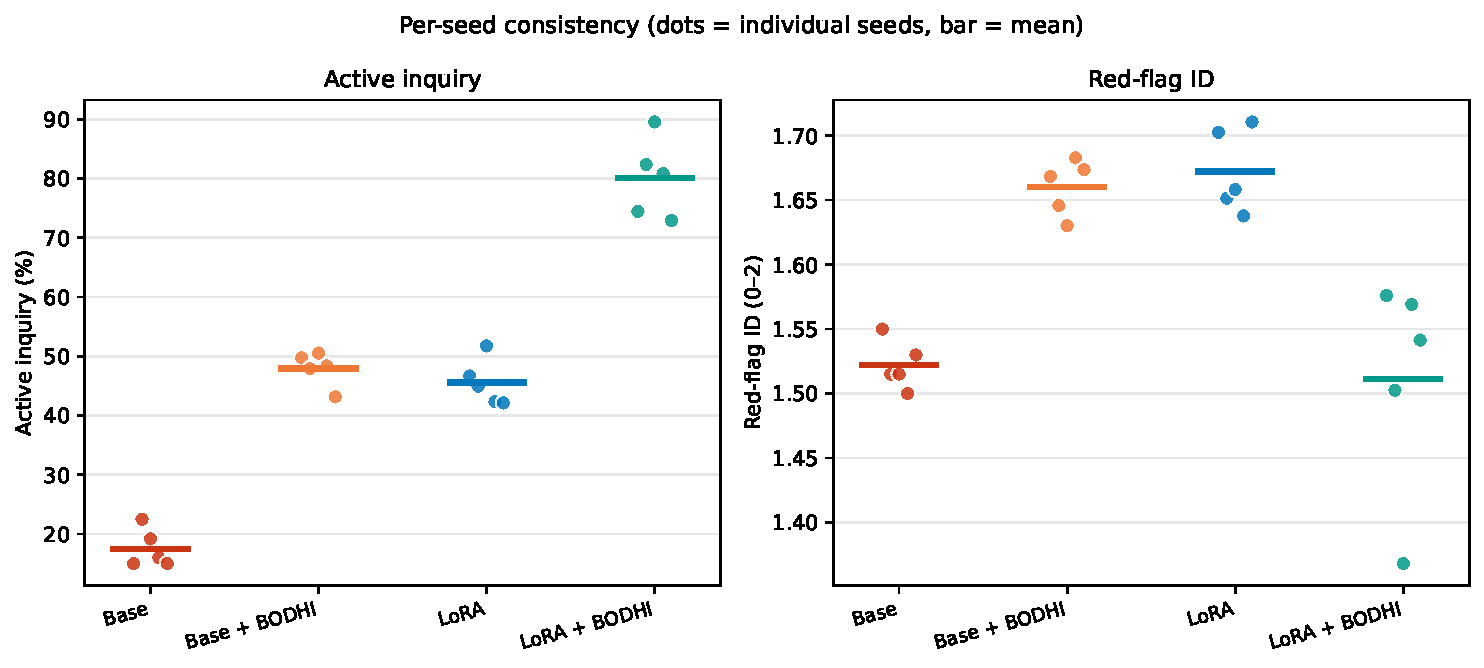
\includegraphics[width=0.85\linewidth]{figures/epistemic_seeds.pdf}
\caption{Per-seed results for active inquiry rate and red-flag identification. Each dot is one of the 5 independent seeds; horizontal tick marks show the cross-seed mean. The between-condition effect is large relative to between-seed variance for both metrics.}
\label{fig:seeds}
\end{figure}

\section{Hyperparameters}
\label{app:hparams}

\begin{table}[t]
\centering
\caption{Training and evaluation configuration.}
\begin{tabular}{ll}
\toprule
Parameter & Value \\
\midrule
Base model & google/medgemma-27b-text-it \\
LoRA rank $r$ & 16 \\
LoRA $\alpha$ & 32 \\
LoRA dropout & 0.05 \\
Target modules & \texttt{\{q,k,v,o,gate,up,down\}\_proj} \\
Epochs & 3 \\
Effective batch size & 16 (2/device $\times$ 8 accum.) \\
Learning rate & $10^{-4}$ (cosine, 5\% warmup) \\
Max sequence length & 4096 \\
Precision & bfloat16 \\
Training hardware & $8\times$ TPU v6e (FSDPv2) \\
Eval hardware & A100-80GB (Modal) \\
vLLM version & $\geq$0.6.5, $<$0.10 (0.6.x series) \\
Filter grader & Qwen/Qwen2.5-14B-Instruct \\
Eval grader & Llama-3.1-8B-Instruct \\
Seeds & 42, 7, 13, 99, 101 \\
Raw traces & 4,000 \\
Filtered traces/seed & ${\sim}$2,800 train + ${\sim}$310 val \\
Eval prompts/seed & 200 (from 1,000 \hbhard{}) \\
\bottomrule
\end{tabular}
\end{table}

\begin{figure}[H]
\centering
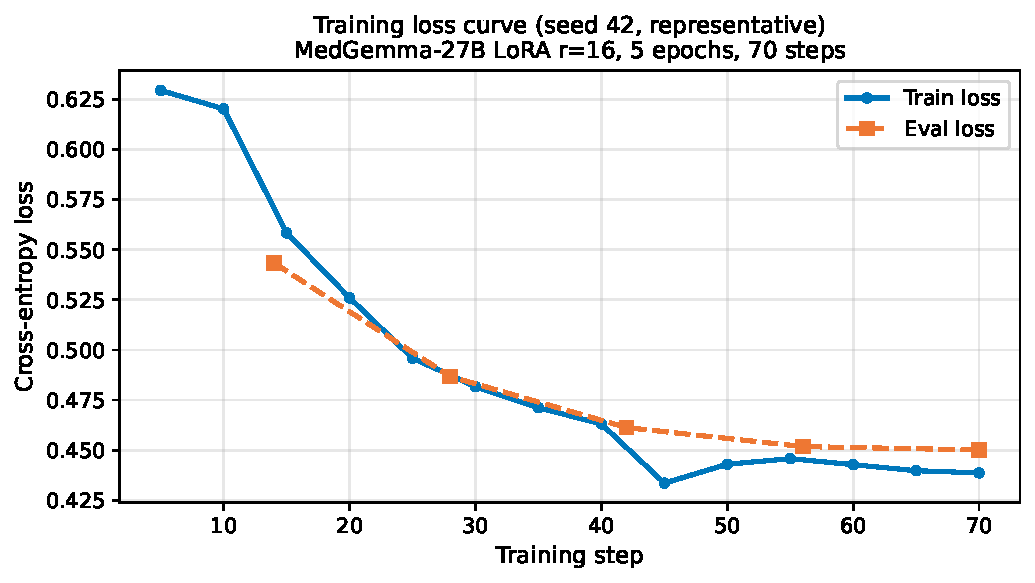
\includegraphics[width=0.7\linewidth]{figures/training_loss_seed42.pdf}
\caption{Training and evaluation loss for seed 42 (representative). Train loss decreases from ${\sim}$0.63 to ${\sim}$0.49 over 70 steps (3 epochs); eval loss checkpoints at steps 14, 42, 70. Loss values for all other seeds were within ${\pm}0.02$ of seed~42's trajectory (not available locally at writing time; stored on GCS).}
\label{fig:trainloss}
\end{figure}

\section{Difficulty Stratification and Axis Breakdown}
\label{app:ushape}

\begin{figure}[H]
\centering
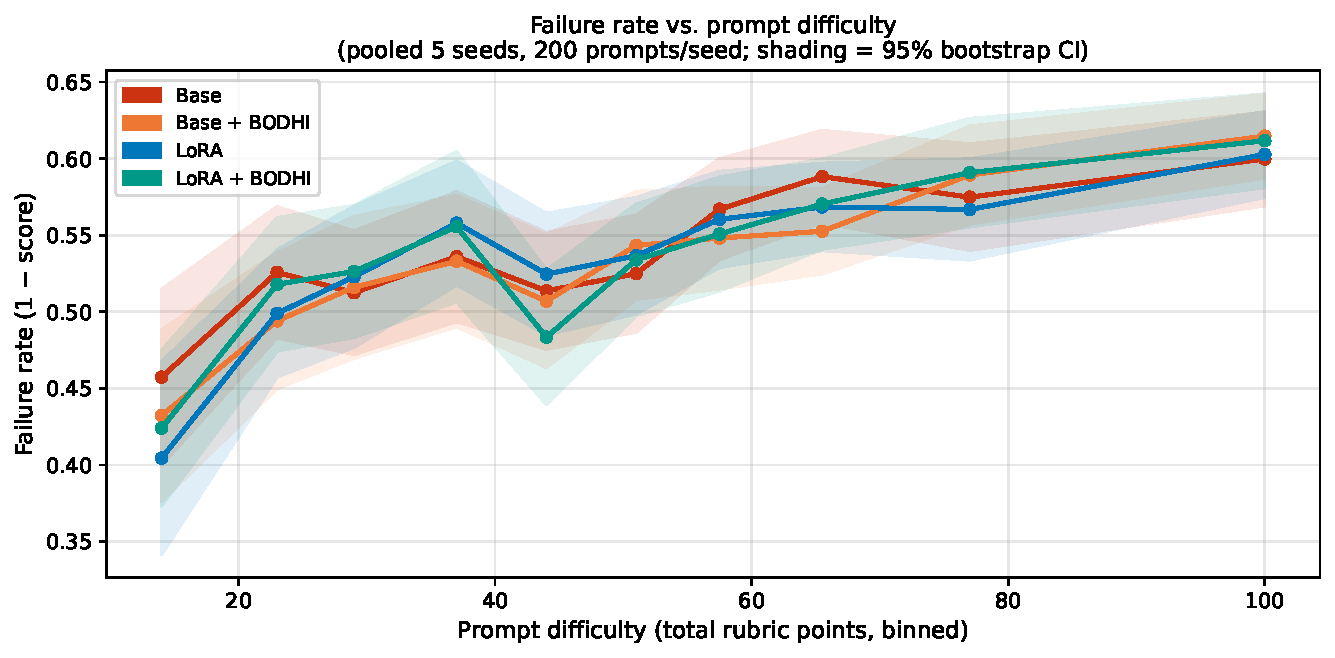
\includegraphics[width=\linewidth]{figures/ushape_difficulty.pdf}
\caption{Failure rate ($1-\text{score}$) vs.\ prompt difficulty, pooled across 5 seeds (1,000 prompts per condition). Difficulty is the sum of positive rubric point values for a prompt (range 5--215, binned into 10 equal-frequency groups). Shading shows 95\% bootstrap CI. Failure rate rises monotonically with difficulty across all conditions. No condition consistently dominates across the full difficulty range, consistent with the adapter modifying communication behavior rather than improving underlying knowledge.}
\label{fig:ushape}
\end{figure}

\begin{figure}[H]
\centering
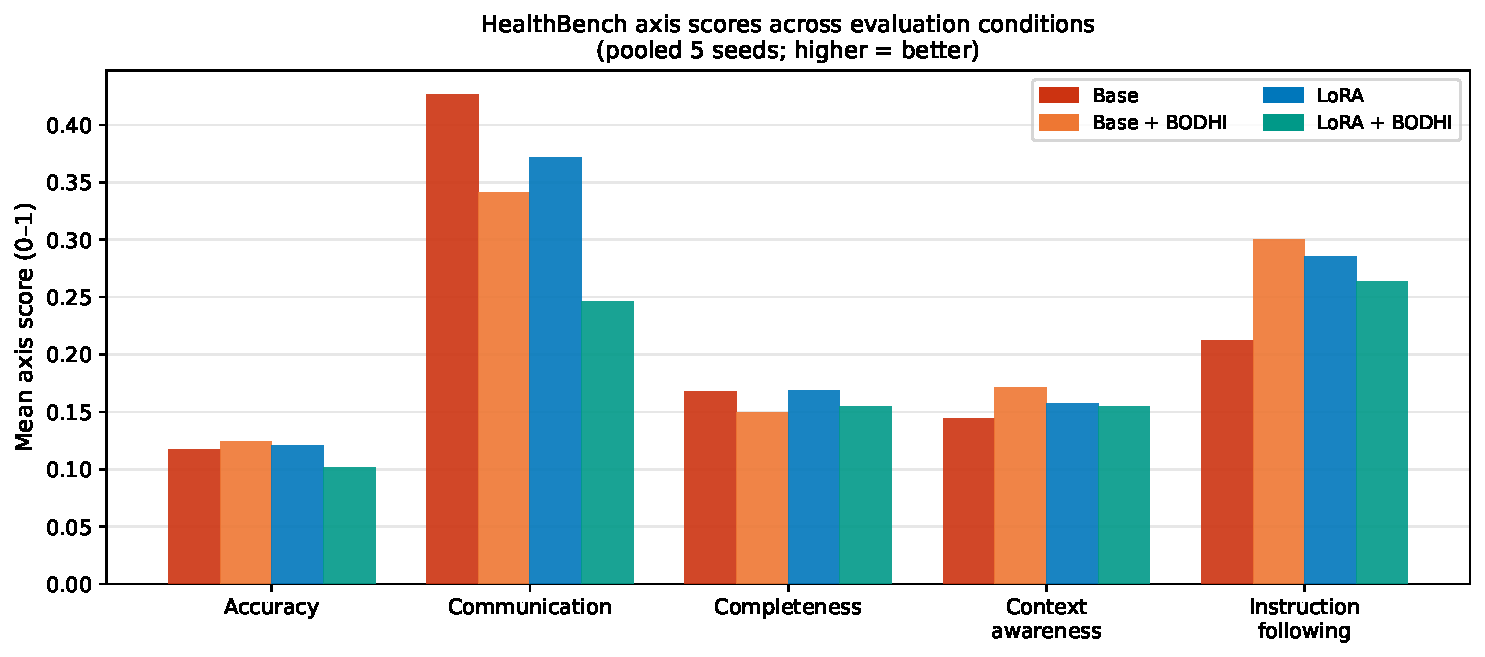
\includegraphics[width=\linewidth]{figures/axis_breakdown.pdf}
\caption{Mean HealthBench score broken down by rubric axis (pooled 5 seeds). The five axes are: accuracy (factual correctness), completeness (coverage of criteria), communication quality (clarity, appropriate tone), context awareness (use of patient context), and instruction following. No axis shows a substantial aggregate difference across conditions, consistent with the non-inferiority result in Table~\ref{tab:main}. The LoRA adapter preserves performance on all five axes, including the safety-sensitive accuracy axis.}
\label{fig:axisbreak}
\end{figure}

\section{Effect Size Forest Plot}
\label{app:forest}

\begin{figure}[H]
\centering
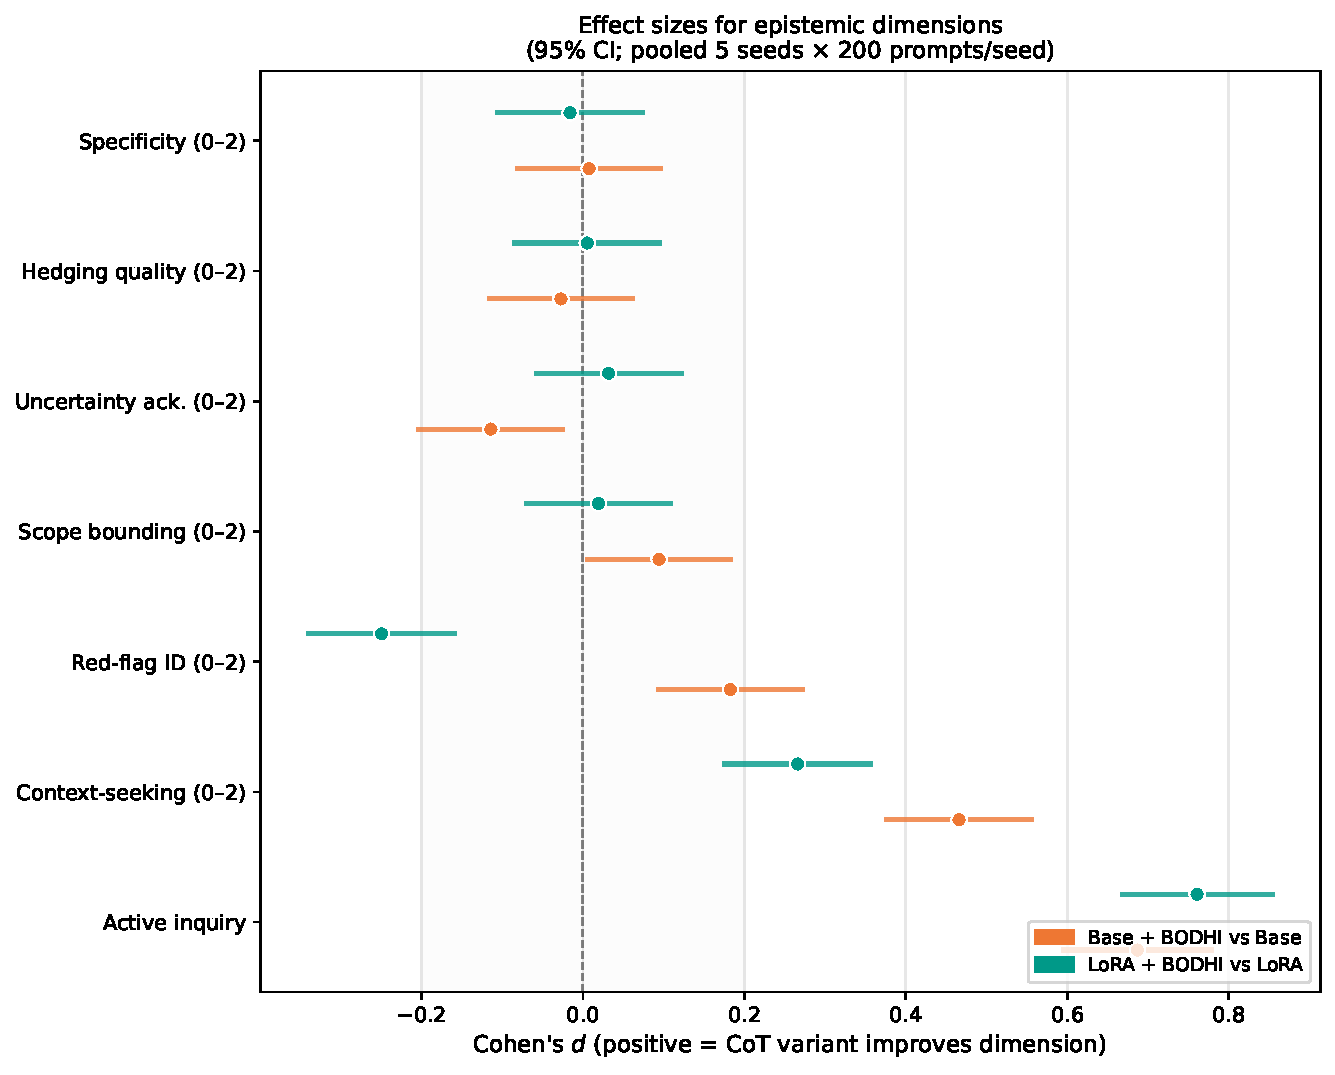
\includegraphics[width=\linewidth]{figures/effect_size_forest.pdf}
\caption{Cohen's $d$ effect sizes for all seven epistemic dimensions. Positive values indicate the CoT variant improves the dimension relative to its baseline; error bars are 95\% confidence intervals under a normal approximation. Both Base+\bodhi{} (orange) and LoRA+\bodhi{} (teal) comparisons are shown. Active inquiry and context-seeking show the largest improvements; red-flag identification is the only dimension that regresses (LoRA+\bodhi{} vs.\ LoRA: $d=-0.25$). The trivial-effect band ($|d|<0.2$) is shaded.}
\label{fig:forest}
\end{figure}

\newpage
\section*{NeurIPS Paper Checklist}

\begin{enumerate}

\item {\bf Claims}
    \item[] Question: Do the main claims made in the abstract and introduction accurately reflect the paper's contributions and scope?
    \item[] Answer: \answerYes{}
    \item[] Justification: The abstract and contributions list frame this explicitly as a proof of concept on one model (MedGemma-27B), one domain (medicine), and one benchmark (\hbhard{}). The Scope paragraph (\S\ref{sec:discussion}) states ``we do not claim this has been validated'' beyond the single setting. Effect sizes are reported at the prompt level ($n\approx1{,}000$, $d=0.20$--$0.63$), not inflated seed-level estimates.
    \item[] Guidelines:
    \begin{itemize}
        \item The answer \answerNA{} means that the abstract and introduction do not include the claims made in the paper.
        \item The abstract and/or introduction should clearly state the claims made, including the contributions made in the paper and important assumptions and limitations. A \answerNo{} or \answerNA{} answer to this question will not be perceived well by the reviewers.
        \item The claims made should match theoretical and experimental results, and reflect how much the results can be expected to generalize to other settings.
        \item It is fine to include aspirational goals as motivation as long as it is clear that these goals are not attained by the paper.
    \end{itemize}

\item {\bf Limitations}
    \item[] Question: Does the paper discuss the limitations of the work performed by the authors?
    \item[] Answer: \answerYes{}
    \item[] Justification: \S\ref{sec:discussion} has explicit paragraphs on single-setting scope (one model, domain, benchmark), self-distillation circularity, LLM-as-judge evaluation, greedy-only decoding, and missing ablations. Appendices~\ref{app:human} and~\ref{app:harm} describe pre-registered studies currently in progress.
    \item[] Guidelines:
    \begin{itemize}
        \item The answer \answerNA{} means that the paper has no limitation while the answer \answerNo{} means that the paper has limitations, but those are not discussed in the paper.
        \item The authors are encouraged to create a separate ``Limitations'' section in their paper.
        \item The paper should point out any strong assumptions and how robust the results are to violations of these assumptions (e.g., independence assumptions, noiseless settings, model well-specification, asymptotic approximations only holding locally). The authors should reflect on how these assumptions might be violated in practice and what the implications would be.
        \item The authors should reflect on the scope of the claims made, e.g., if the approach was only tested on a few datasets or with a few runs. In general, empirical results often depend on implicit assumptions, which should be articulated.
        \item The authors should reflect on the factors that influence the performance of the approach. For example, a facial recognition algorithm may perform poorly when image resolution is low or images are taken in low lighting. Or a speech-to-text system might not be used reliably to provide closed captions for online lectures because it fails to handle technical jargon.
        \item The authors should discuss the computational efficiency of the proposed algorithms and how they scale with dataset size.
        \item If applicable, the authors should discuss possible limitations of their approach to address problems of privacy and fairness.
        \item While the authors might fear that complete honesty about limitations might be used by reviewers as grounds for rejection, a worse outcome might be that reviewers discover limitations that aren't acknowledged in the paper. The authors should use their best judgment and recognize that individual actions in favor of transparency play an important role in developing norms that preserve the integrity of the community. Reviewers will be specifically instructed to not penalize honesty concerning limitations.
    \end{itemize}

\item {\bf Theory assumptions and proofs}
    \item[] Question: For each theoretical result, does the paper provide the full set of assumptions and a complete (and correct) proof?
    \item[] Answer: \answerNA{}
    \item[] Justification: The paper makes no theoretical claims and contains no theorems or proofs.
    \item[] Guidelines:
    \begin{itemize}
        \item The answer \answerNA{} means that the paper does not include theoretical results.
        \item All the theorems, formulas, and proofs in the paper should be numbered and cross-referenced.
        \item All assumptions should be clearly stated or referenced in the statement of any theorems.
        \item The proofs can either appear in the main paper or the supplemental material, but if they appear in the supplemental material, the authors are encouraged to provide a short proof sketch to provide intuition.
        \item Inversely, any informal proof provided in the core of the paper should be complemented by formal proofs provided in appendix or supplemental material.
        \item Theorems and Lemmas that the proof relies upon should be properly referenced.
    \end{itemize}

    \item {\bf Experimental result reproducibility}
    \item[] Question: Does the paper fully disclose all the information needed to reproduce the main experimental results of the paper to the extent that it affects the main claims and/or conclusions of the paper (regardless of whether the code and data are provided or not)?
    \item[] Answer: \answerYes{}
    \item[] Justification: Full hyperparameters are in Appendix~\ref{app:hparams}. The pipeline is deterministic given fixed seeds (greedy decoding, seeded LoRA init, seeded data order, seeded eval draws). Hardware is specified (TPU v6e-8 for training, A100-80GB for evaluation). Code and trained adapters are at \url{https://anonymous.4open.science/r/bodhi-lora-CEB5}.
    \item[] Guidelines:
    \begin{itemize}
        \item The answer \answerNA{} means that the paper does not include experiments.
        \item If the paper includes experiments, a \answerNo{} answer to this question will not be perceived well by the reviewers: Making the paper reproducible is important, regardless of whether the code and data are provided or not.
        \item If the contribution is a dataset and\slash or model, the authors should describe the steps taken to make their results reproducible or verifiable.
        \item Depending on the contribution, reproducibility can be accomplished in various ways. For example, if the contribution is a novel architecture, describing the architecture fully might suffice, or if the contribution is a specific model and empirical evaluation, it may be necessary to either make it possible for others to replicate the model with the same dataset, or provide access to the model. In general. releasing code and data is often one good way to accomplish this, but reproducibility can also be provided via detailed instructions for how to replicate the results, access to a hosted model (e.g., in the case of a large language model), releasing of a model checkpoint, or other means that are appropriate to the research performed.
        \item While NeurIPS does not require releasing code, the conference does require all submissions to provide some reasonable avenue for reproducibility, which may depend on the nature of the contribution. For example
        \begin{enumerate}
            \item If the contribution is primarily a new algorithm, the paper should make it clear how to reproduce that algorithm.
            \item If the contribution is primarily a new model architecture, the paper should describe the architecture clearly and fully.
            \item If the contribution is a new model (e.g., a large language model), then there should either be a way to access this model for reproducing the results or a way to reproduce the model (e.g., with an open-source dataset or instructions for how to construct the dataset).
            \item We recognize that reproducibility may be tricky in some cases, in which case authors are welcome to describe the particular way they provide for reproducibility. In the case of closed-source models, it may be that access to the model is limited in some way (e.g., to registered users), but it should be possible for other researchers to have some path to reproducing or verifying the results.
        \end{enumerate}
    \end{itemize}

\item {\bf Open access to data and code}
    \item[] Question: Does the paper provide open access to the data and code, with sufficient instructions to faithfully reproduce the main experimental results, as described in supplemental material?
    \item[] Answer: \answerYes{}
    \item[] Justification: Code, trained LoRA adapters (5 seeds), and evaluation scripts are at \url{https://anonymous.4open.science/r/bodhi-lora-CEB5}. HealthBench is publicly available from OpenAI. MedGemma-27B requires a standard HuggingFace gated-model access request; Qwen and Llama graders are fully open.
    \item[] Guidelines:
    \begin{itemize}
        \item The answer \answerNA{} means that paper does not include experiments requiring code.
        \item Please see the NeurIPS code and data submission guidelines (\url{https://neurips.cc/public/guides/CodeSubmissionPolicy}) for more details.
        \item While we encourage the release of code and data, we understand that this might not be possible, so \answerNo{} is an acceptable answer. Papers cannot be rejected simply for not including code, unless this is central to the contribution (e.g., for a new open-source benchmark).
        \item The instructions should contain the exact command and environment needed to run to reproduce the results. See the NeurIPS code and data submission guidelines (\url{https://neurips.cc/public/guides/CodeSubmissionPolicy}) for more details.
        \item The authors should provide instructions on data access and preparation, including how to access the raw data, preprocessed data, intermediate data, and generated data, etc.
        \item The authors should provide scripts to reproduce all experimental results for the new proposed method and baselines. If only a subset of experiments are reproducible, they should state which ones are omitted from the script and why.
        \item At submission time, to preserve anonymity, the authors should release anonymized versions (if applicable).
        \item Providing as much information as possible in supplemental material (appended to the paper) is recommended, but including URLs to data and code is permitted.
    \end{itemize}

\item {\bf Experimental setting/details}
    \item[] Question: Does the paper specify all the training and test details (e.g., data splits, hyperparameters, how they were chosen, type of optimizer) necessary to understand the results?
    \item[] Answer: \answerYes{}
    \item[] Justification: \S\ref{sec:method} describes trace generation, grading, filtering, LoRA fine-tuning, and evaluation. Appendix~\ref{app:hparams} contains a complete hyperparameter table (rank, $\alpha$, dropout, batch size, LR schedule, sequence length, hardware, seeds, grader models).
    \item[] Guidelines:
    \begin{itemize}
        \item The answer \answerNA{} means that the paper does not include experiments.
        \item The experimental setting should be presented in the core of the paper to a level of detail that is necessary to appreciate the results and make sense of them.
        \item The full details can be provided either with the code, in appendix, or as supplemental material.
    \end{itemize}

\item {\bf Experiment statistical significance}
    \item[] Question: Does the paper report error bars suitably and correctly defined or other appropriate information about the statistical significance of the experiments?
    \item[] Answer: \answerYes{}
    \item[] Justification: Table~\ref{tab:main} reports 95\% CIs across 5 seeds. Table~\ref{tab:epistemic} reports cross-seed std as subscripts. All epistemic virtue claims use prompt-level two-sample $t$-tests ($n\approx985$--$998$ per condition, pooled across 5 seeds; seeds draw without replacement within-seed but independently across seeds, introducing some prompt overlap that does not affect binary significance conclusions at reported effect sizes), with Cohen's $d$ and exact $p$-values. The statistical method and its limitations are stated explicitly in \S\ref{sec:results}.
    \item[] Guidelines:
    \begin{itemize}
        \item The answer \answerNA{} means that the paper does not include experiments.
        \item The authors should answer \answerYes{} if the results are accompanied by error bars, confidence intervals, or statistical significance tests, at least for the experiments that support the main claims of the paper.
        \item The factors of variability that the error bars are capturing should be clearly stated (for example, train/test split, initialization, random drawing of some parameter, or overall run with given experimental conditions).
        \item The method for calculating the error bars should be explained (closed form formula, call to a library function, bootstrap, etc.)
        \item The assumptions made should be given (e.g., Normally distributed errors).
        \item It should be clear whether the error bar is the standard deviation or the standard error of the mean.
        \item It is OK to report 1-sigma error bars, but one should state it. The authors should preferably report a 2-sigma error bar than state that they have a 96\% CI, if the hypothesis of Normality of errors is not verified.
        \item For asymmetric distributions, the authors should be careful not to show in tables or figures symmetric error bars that would yield results that are out of range (e.g., negative error rates).
        \item If error bars are reported in tables or plots, the authors should explain in the text how they were calculated and reference the corresponding figures or tables in the text.
    \end{itemize}

\item {\bf Experiments compute resources}
    \item[] Question: For each experiment, does the paper provide sufficient information on the computer resources (type of compute workers, memory, time of execution) needed to reproduce the experiments?
    \item[] Answer: \answerYes{}
    \item[] Justification: Training: $8\times$ TPU v6e (256\,GB HBM, FSDPv2), ${\sim}$4\,h/seed $\times$ 5 seeds. Evaluation: A100-80GB via Modal, ${\sim}$2\,h/seed. Hardware is stated in Appendix~\ref{app:hparams} and the Reproducibility Statement.
    \item[] Guidelines:
    \begin{itemize}
        \item The answer \answerNA{} means that the paper does not include experiments.
        \item The paper should indicate the type of compute workers CPU or GPU, internal cluster, or cloud provider, including relevant memory and storage.
        \item The paper should provide the amount of compute required for each of the individual experimental runs as well as estimate the total compute.
        \item The paper should disclose whether the full research project required more compute than the experiments reported in the paper (e.g., preliminary or failed experiments that didn't make it into the paper).
    \end{itemize}

\item {\bf Code of ethics}
    \item[] Question: Does the research conducted in the paper conform, in every respect, with the NeurIPS Code of Ethics \url{https://neurips.cc/public/EthicsGuidelines}?
    \item[] Answer: \answerYes{}
    \item[] Justification: No patient data is used. Training data is from a public benchmark (HealthBench). The Ethics Statement addresses the primary risk (excessive hedging delaying emergency care) and states the model is a research contribution not intended for unsupervised clinical deployment.
    \item[] Guidelines:
    \begin{itemize}
        \item The answer \answerNA{} means that the authors have not reviewed the NeurIPS Code of Ethics.
        \item If the authors answer \answerNo, they should explain the special circumstances that require a deviation from the Code of Ethics.
        \item The authors should make sure to preserve anonymity (e.g., if there is a special consideration due to laws or regulations in their jurisdiction).
    \end{itemize}

\item {\bf Broader impacts}
    \item[] Question: Does the paper discuss both potential positive societal impacts and negative societal impacts of the work performed?
    \item[] Answer: \answerYes{}
    \item[] Justification: The Ethics Statement discusses both positive impact (more calibrated medical AI) and the primary negative risk (excessive hedging delaying emergency care). Appendix~\ref{app:harm} pre-registers clinician review on chest pain, anaphylaxis, suicide risk, and drug-allergy scenarios.
    \item[] Guidelines:
    \begin{itemize}
        \item The answer \answerNA{} means that there is no societal impact of the work performed.
        \item If the authors answer \answerNA{} or \answerNo, they should explain why their work has no societal impact or why the paper does not address societal impact.
        \item Examples of negative societal impacts include potential malicious or unintended uses (e.g., disinformation, generating fake profiles, surveillance), fairness considerations (e.g., deployment of technologies that could make decisions that unfairly impact specific groups), privacy considerations, and security considerations.
        \item The conference expects that many papers will be foundational research and not tied to particular applications, let alone deployments. However, if there is a direct path to any negative applications, the authors should point it out. For example, it is legitimate to point out that an improvement in the quality of generative models could be used to generate Deepfakes for disinformation. On the other hand, it is not needed to point out that a generic algorithm for optimizing neural networks could enable people to train models that generate Deepfakes faster.
        \item The authors should consider possible harms that could arise when the technology is being used as intended and functioning correctly, harms that could arise when the technology is being used as intended but gives incorrect results, and harms following from (intentional or unintentional) misuse of the technology.
        \item If there are negative societal impacts, the authors could also discuss possible mitigation strategies (e.g., gated release of models, providing defenses in addition to attacks, mechanisms for monitoring misuse, mechanisms to monitor how a system learns from feedback over time, improving the efficiency and accessibility of ML).
    \end{itemize}

\item {\bf Safeguards}
    \item[] Question: Does the paper describe safeguards that have been put in place for responsible release of data or models that have a high risk for misuse (e.g., pre-trained language models, image generators, or scraped datasets)?
    \item[] Answer: \answerYes{}
    \item[] Justification: The adapter increases epistemic caution rather than enabling harmful outputs. It requires the gated base model (MedGemma-27B) and is released under the same terms. The paper states it is not for unsupervised clinical deployment.
    \item[] Guidelines:
    \begin{itemize}
        \item The answer \answerNA{} means that the paper poses no such risks.
        \item Released models that have a high risk for misuse or dual-use should be released with necessary safeguards to allow for controlled use of the model, for example by requiring that users adhere to usage guidelines or restrictions to access the model or implementing safety filters.
        \item Datasets that have been scraped from the Internet could pose safety risks. The authors should describe how they avoided releasing unsafe images.
        \item We recognize that providing effective safeguards is challenging, and many papers do not require this, but we encourage authors to take this into account and make a best faith effort.
    \end{itemize}

\item {\bf Licenses for existing assets}
    \item[] Question: Are the creators or original owners of assets (e.g., code, data, models), used in the paper, properly credited and are the license and terms of use explicitly mentioned and properly respected?
    \item[] Answer: \answerYes{}
    \item[] Justification: HealthBench \citep{healthbench2025}: MIT license (OpenAI). MedGemma-27B \citep{medgemma2025}: Health AI Developer Foundations terms (Google). Qwen2.5-14B: Qwen License. Llama-3.1-8B: Meta Llama 3.1 Community License. LoRA \citep{hu2022lora}: Apache 2.0. All used within stated terms.
    \item[] Guidelines:
    \begin{itemize}
        \item The answer \answerNA{} means that the paper does not use existing assets.
        \item The authors should cite the original paper that produced the code package or dataset.
        \item The authors should state which version of the asset is used and, if possible, include a URL.
        \item The name of the license (e.g., CC-BY 4.0) should be included for each asset.
        \item For scraped data from a particular source (e.g., website), the copyright and terms of service of that source should be provided.
        \item If assets are released, the license, copyright information, and terms of use in the package should be provided. For popular datasets, \url{paperswithcode.com/datasets} has curated licenses for some datasets. Their licensing guide can help determine the license of a dataset.
        \item For existing datasets that are re-packaged, both the original license and the license of the derived asset (if it has changed) should be provided.
        \item If this information is not available online, the authors are encouraged to reach out to the asset's creators.
    \end{itemize}

\item {\bf New assets}
    \item[] Question: Are new assets introduced in the paper well documented and is the documentation provided alongside the assets?
    \item[] Answer: \answerYes{}
    \item[] Justification: Five trained LoRA adapters are released at \url{https://anonymous.4open.science/r/bodhi-lora-CEB5} with a model card covering training procedure, intended use, limitations, and license. Evaluation code and grading scripts are included with usage instructions.
    \item[] Guidelines:
    \begin{itemize}
        \item The answer \answerNA{} means that the paper does not release new assets.
        \item Researchers should communicate the details of the dataset\slash code\slash model as part of their submissions via structured templates. This includes details about training, license, limitations, etc.
        \item The paper should discuss whether and how consent was obtained from people whose asset is used.
        \item At submission time, remember to anonymize your assets (if applicable). You can either create an anonymized URL or include an anonymized zip file.
    \end{itemize}

\item {\bf Crowdsourcing and research with human subjects}
    \item[] Question: For crowdsourcing experiments and research with human subjects, does the paper include the full text of instructions given to participants and screenshots, if applicable, as well as details about compensation (if any)?
    \item[] Answer: \answerYes{}
    \item[] Justification: Appendix~\ref{app:human} describes the physician validation protocol in full: grading criteria, per-criterion format, confidence scale, and tie-breaking procedure. Participating physicians are co-authors; no separate compensation applies beyond authorship.
    \item[] Guidelines:
    \begin{itemize}
        \item The answer \answerNA{} means that the paper does not involve crowdsourcing nor research with human subjects.
        \item Including this information in the supplemental material is fine, but if the main contribution of the paper involves human subjects, then as much detail as possible should be included in the main paper.
        \item According to the NeurIPS Code of Ethics, workers involved in data collection, curation, or other labor should be paid at least the minimum wage in the country of the data collector.
    \end{itemize}

\item {\bf Institutional review board (IRB) approvals or equivalent for research with human subjects}
    \item[] Question: Does the paper describe potential risks incurred by study participants, whether such risks were disclosed to the subjects, and whether Institutional Review Board (IRB) approvals (or an equivalent approval/review based on the requirements of your country or institution) were obtained?
    \item[] Answer: \answerNo{}
    \item[] Justification: The physician validation (Appendix~\ref{app:human}) involves co-authors grading AI-generated text against publicly available rubrics. No patient data or patient contact is involved. A formal IRB determination is being sought at the participating institutions for camera-ready.
    \item[] Guidelines:
    \begin{itemize}
        \item The answer \answerNA{} means that the paper does not involve crowdsourcing nor research with human subjects.
        \item Depending on the country in which research is conducted, IRB approval (or equivalent) may be required for any human subjects research. If you obtained IRB approval, you should clearly state this in the paper.
        \item We recognize that the procedures for this may vary significantly between institutions and locations, and we expect authors to adhere to the NeurIPS Code of Ethics and the guidelines for their institution.
        \item For initial submissions, do not include any information that would break anonymity (if applicable), such as the institution conducting the review.
    \end{itemize}

\item {\bf Declaration of LLM usage}
    \item[] Question: Does the paper describe the usage of LLMs if it is an important, original, or non-standard component of the core methods in this research? Note that if the LLM is used only for writing, editing, or formatting purposes and does \emph{not} impact the core methodology, scientific rigor, or originality of the research, declaration is not required.
    \item[] Answer: \answerYes{}
    \item[] Justification: LLMs are central to the methodology. MedGemma-27B-text-it is the base model being adapted; Qwen/Qwen2.5-14B-Instruct is the filter grader (\S\ref{sec:method}); Llama-3.1-8B-Instruct is the evaluation grader (\S\ref{sec:eval}). All model identifiers and versions are in Appendix~\ref{app:hparams}.
    \item[] Guidelines:
    \begin{itemize}
        \item The answer \answerNA{} means that the core method development in this research does not involve LLMs as any important, original, or non-standard components.
        \item Please refer to our LLM policy in the NeurIPS handbook for what should or should not be described.
    \end{itemize}

\end{enumerate}


\end{document}
